\documentclass{lecturenotes}

\renewcommand{\vecka}{9}
\newcommand{\tema}{Matriser}

\setbeamertemplate{footline}[frame number]
\title[Föreläsningsanteckningar EDA016, 2015]{EDA016 Programmeringsteknik för D}
\subtitle{Läsvecka \vecka: \tema}
\author{Björn Regnell}
\institute{Datavetenskap, LTH}
\date{Lp1-2, HT 2015}

%%%%%%%%%%%%%%%%%%%%%%%%%%%%%%%%%%%%%%

\begin{document}

\frame{\titlepage}
\setnextsection{\vecka}
\section[Vecka \vecka: \tema]{\tema}
\frame{\tableofcontents}

\subsection{Att göra denna vecka}
\begin{Slide}{Att göra i Vecka \vecka: Förstå matriser. \\ Komma ikapp med övningar etc.}
\begin{enumerate}
\item Läs följande kapitel i kursboken:  8.6-8.7 \\  
Begrepp: matris, vektor av vektorer, matrisindexering, rader, kolonner/kolumner, nästlade for-satser
\item Gör övning 8: matriser, \code{StringBuilder}
\item Förslag: skriv kontrollskrivningsuppgiften själv i Eclipse. \\ {\small Övning: implementera en klass \code{ChordView} som har ett \code{Chord} och ett \code{SimpleWindow} som attribut och metoden \code{draw()} som ritar ackordbilder. Skapa privata hjälpmetoder för olika delar av bilden (rutnät, band noll, kvadrat för nedtryckt sträng, etc.)}
\item Träffas i samarbetsgrupper och hjälp varandra 
\item Gör Lab 7: Maze
\end{enumerate}
\end{Slide}

\subsection{Repetition: Vektorer}
\begin{Slide}{Repetition: Vektorer}\footnotesize
\begin{itemize}
\item Deklarera en vektor-referensvariabel: \\ \code{int[] v;     // ej intialliserad}
\item Vektorer är (speciella) objekt; vi kan använda \code{null} och \code{new}: \\ 
           \code{v = null;   // inga element är allokerede förrän vi gör new} \\
           \code{v = new int[5];  // allokera plats för 5 heltal, init 0}
\item Deklarera, allokera och initialisera på en och samma gång: \\
           \code{int[] v = new int[5];   //  elementen initialisers med nollor}
\item Indexera i en vektor: \\ 
    \code{int firstElement = v[0];  //indexering från noll} \\
    \code{int lastElement = v[4];}   \\
    \code{int error = v[5];  //ger ArrayIndexOutOfBoundsException}   \\    
\item Elementen kan användas som ''vanliga'' variabler: \\ \code{v[3] = v[3] + 1;   //öka fjärde elementet med 1}
\item Deklarera referens, allokera och initialisera vektor från konstanter: \\
\code!int[] xs = new int[] {42, 43, 44, 45};!\\
\code!int[] ys = {42, 43, 44, 45};  // kortform av ovan!

\end{itemize}
\end{Slide}

\begin{Slide}{Övning: Vektorer}
Rita bild av minnet efter rad 1 och rad 4.
\begin{Code}[numberstyle=,numbers=left]
    int[] v = new int[5];
    for (int i = 0; i < 5; i++){
        v[i] = 2 * i + 1;
    }
    System.out.println(v[0]);
    System.out.println(v[v[0]]);
    System.out.println(v[v[v[0]]]);
    System.out.println(v[v[v[v[0]]]]); 
\end{Code}
Vad skrivs ut på raderna 5-8? 
\end{Slide}

\subsection{Skapa matriser}

\begin{Slide}{Vad är en matris?}
\begin{itemize}
\item En matris är ett tvådimensionellt fält; en tabell; ett ''rutnät''.
\item Exempel 5x4-matris: \\ \vspace{1em}
\begin{tabular}{lllll}
kolumn                     & 0                       & 1                        & 2                        & 3                       \\ \cline{2-5} 
\multicolumn{1}{l|}{rad 0} & \multicolumn{1}{l|}{7}  & \multicolumn{1}{l|}{9}   & \multicolumn{1}{l|}{123} & \multicolumn{1}{l|}{41} \\ \cline{2-5} 
\multicolumn{1}{l|}{rad 1} & \multicolumn{1}{l|}{22} & \multicolumn{1}{l|}{-18} & \multicolumn{1}{l|}{12}  & \multicolumn{1}{l|}{2}  \\ \cline{2-5} 
\multicolumn{1}{l|}{rad 2} & \multicolumn{1}{l|}{11} & \multicolumn{1}{l|}{16}  & \multicolumn{1}{l|}{-4}  & \multicolumn{1}{l|}{0}  \\ \cline{2-5} 
\multicolumn{1}{l|}{rad 3} & \multicolumn{1}{l|}{1}  & \multicolumn{1}{l|}{1}   & \multicolumn{1}{l|}{1}   & \multicolumn{1}{l|}{1}  \\ \cline{2-5} 
\multicolumn{1}{l|}{rad 4} & \multicolumn{1}{l|}{2}  & \multicolumn{1}{l|}{2}   & \multicolumn{1}{l|}{2}   & \multicolumn{1}{l|}{2}  \\ \cline{2-5} 
\end{tabular}
\end{itemize}
\end{Slide}

\begin{Slide}{Deklarera och allokera en matris i Java med vektorer}
I Java kan matriser representeras som vektorer av vektorer: \\ \vspace{1em}
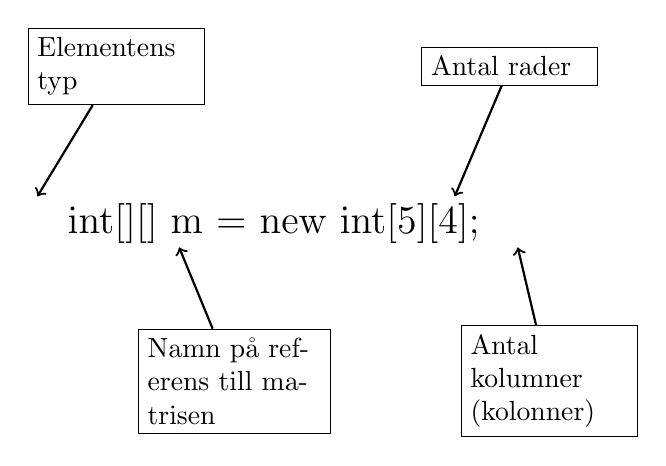
\begin{tikzpicture}
\node[draw, text width=2.2cm] (ref) at (-0.5,-2)     {Namn på referens till matrisen};
\draw[->, thick] (ref) -- (-1.2,-0.3);

\node[draw, text width=2cm] (typ) at (-2,2)     {Elementens typ};
\draw[->, thick] (typ) -- (-3,0.35);

\node[draw, text width=2cm] (typ) at (3,2)     {Antal rader};
\draw[->, thick] (typ) -- (2.3,0.35);

\node[draw, text width=2cm] (typ) at (3.5,-2)     {Antal kolumner (kolonner)};
\draw[->, thick] (typ) -- (3.1,-0.3);

\node {\Large\code{int[][] m = new int[5][4];}};
\end{tikzpicture}
\end{Slide}

\subsection{Använda matriser}
\begin{Slide}{Använda matriser (vektorer av vektorer)}\footnotesize
\begin{itemize}
\item Indexera i en matris: \\ \vspace{1em}
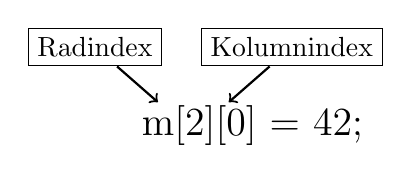
\begin{tikzpicture}
\node[draw] (ref) at (-2,1)     {Radindex};
\draw[->, thick] (ref) -- (-1.2,0.3);

\node[draw] (typ) at (0.5,1)     {Kolumnindex};
\draw[->, thick] (typ) -- (-0.3,0.3);

\node {\Large\code{m[2][0] = 42;}};
\end{tikzpicture}
\item Ta reda på antalet rader: \\ \code{m.length}
\item Ta reda på antalet kolumner på tredje raden: \\ \code{m[2].length} 
\item Man \emph{kan} ha varierande radlängd, genom att allokera resp radvektor enskilt, men det är ganska ovanligt: \\ 
   \code!m[1] = new int[] { 42, 43 };! 
\item Man \emph{kan} ha vektorer av vektorer av vektorer i godtyckligt djup, t.ex. för att representera en kub (3 dimensioner), men det är inte så vanligt. 
\end{itemize}
\end{Slide}

\begin{Slide}{Deklarera, Allokera, Tilldela, Gå igenom alla}
  \begin{minipage}{0.7\linewidth}   
\footnotesize\href{https://github.com/bjornregnell/lth-eda016-2015/tree/master/lectures/examples/eclipse-ws/lecture-examples/src/week09}{lecture-examples/src/week09/matrix}:

\begin{Code}[basicstyle=\ttfamily\fontsize{7}{8}\selectfont, numberstyle=,numbers=left]
// deklaration och allokering:
int m[][] = new int[5][4];
        
// tilldelning:
m[0][0] = 42;
m[1] = new int[] { 42, 43, 44, 45 };

// avvikande antal kolumner ok i Java:
m[3] = new int[] { -1, -2 }; 
        
System.out.println("Matrisen m:");

// nästlade for-loopar:        
for (int row = 0; row < m.length; row++) {
    for (int col = 0; col < m[row].length; col++) {
        System.out.print(m[row][col] + " ");
    }
    System.out.println();
}
\end{Code}
\end{minipage}
\hspace{0.5cm}
\begin{minipage}[t]{0.2\linewidth}   
\begin{verbatim}
Matrisen m:
42 0 0 0 
42 43 44 45 
0 0 0 0 
-1 -2 
0 0 0 0 
\end{verbatim}
  \end{minipage}
\end{Slide}

\begin{Slide}{Beräkna radsummorna}
\footnotesize\href{https://github.com/bjornregnell/lth-eda016-2015/tree/master/lectures/examples/eclipse-ws/lecture-examples/src/week09}{lecture-examples/src/week09/matrix}:
\begin{Code}[numberstyle=,numbers=left]
        int[][] matrix = { { 1, 2, 3, 4 }, { 5, 6, 7, 8 }, {9, 10, 11, 12} };
        
        System.out.println("\nRadsummorna i matrix:");
        for (int row = 0; row < matrix.length; row++) {
            int sum = 0;
            for (int col = 0; col < matrix[row].length; col++) {
                sum = sum + matrix[row][col];
            }
            System.out.println("row" + "[" + row + "]: " + sum);
        }        
\end{Code}
\begin{verbatim}
Radsummorna i matrix:
row[0]: 10
row[1]: 26
row[2]: 42
\end{verbatim}
\end{Slide}

\begin{Slide}{Användning av nästlade for-satser och matriser}
\Alert{Kunskapen behövs på övn8, lab7, lab10, lab11 och tenta!}\\ \vspace{1em}
Pseudokod:
\begin{verbatim}
för varje rad
  för varje kolumn
     bearbeta m[rad][kolumn]
\end{verbatim}
Implementation i Java:
\begin{Code}
        // deklarera och initisalisera m
        for (int row = 0; row < matrix.length; row++) {
            // deklarera och initisalisera
            for (int col = 0; col < matrix[row].length; col++) {
                 // bearbeta varje element m[rad][kolumn]
            }
           // bearbeta varje rad vid behov
        }
\end{Code}
\end{Slide}

\begin{Slide}{Övning: matris för schakbräde}
Deklarera och skapa en matris som representerar ett schackbräde med 8x8 rutor. På rutorna ska man kunna placera schackpjäser som beskrivs av klassen ChessPiece.
\end{Slide}

\begin{Slide}{Designexempel: Tre-i-rad}
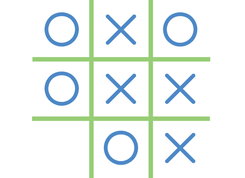
\includegraphics{img/tictactoe}

\href{https://en.wikipedia.org/wiki/Tic-tac-toe}{Tic Tac Toe}
\end{Slide}

\begin{Slide}{Tre-i-rad med MVC-designmönstret}
Vi ska använda ett designmönstret som kallas \textit{Model-View-Controller} där vi har dessa tre klasser med sina respektive speciella ansvar:
\begin{itemize}
\item \Emph{Model}: Har hand om spelets datamodell, här spelbrädet och pjäsernas placering. Har metoder som kan avläsa och ändra data om spelet.
\item \Emph{View}: Har hand om den för användaren synliga representationen av modellen och användarens interaktion med modellen. Visar brädet och läser användarens input.
\item \Emph{Controller}: Styr spelet enligt dess regler och har hand om logiken för en spelomgång.
\end{itemize}
Idén är att man renodlar ansvaret så att man lätt kan ändra och byta delar utan att det påverkar de andra delarna. 
\end{Slide}

\begin{Slide}{Implementera \texttt{Model} enligt specifikationen}
\vspace{-2em}
\begin{ClassSpec}{}
/** Skapar en modell av ett Tre-i-rad-spel med ett tomt bräde */
Model();

/** Tömmer brädet från pjäser */
void clear();

/** Returnerar pjäsen på platsen (row, col): X eller 0 eller blank om ledig  */
char getMark(int row, int col);

/** Returnerar true om platsen är ledig */
boolean isFree(int row, int col);

/** Returnerar true om platsen är innanför brädets rader och kolumner */
boolean isInside(int row, int col);

/** Returnerar true om alla platserna är upptagna */
boolean isFull();

/** Placerar en ring på platsen (row, col) */
void markNought(int row, int col);

/** Placerar en kryss på platsen (row, col) */
void markCross(int row, int col);

/** Returnerar X om kryss är vinnare, 0 om ring är vinnare och blank vinnare saknas */
char getWinner();
\end{ClassSpec}
\footnotesize\vspace{-0.2em} Vilka \Emph{attribut} behöver vi? 
\end{Slide}

\begin{Slide}{Klassen \texttt{Model} med tomma metodkroppar: Gör klart!}

\begin{Code}
public class Model {
    private char[][] board = new char [3][3];
    
    public Model(){    }
    
    public void clear(){    }
    
    public char getMark(int row, int col){    }
    
    public boolean isFree(int row, int col){    }

    public boolean isInside(int row, int col){    }
    
    public boolean isFull(){    }

    public void markNought(int row, int col){    }

    public void markCross(int row, int col){    }
    
    public char getWinner(){    }
}
\end{Code}
\end{Slide}

\begin{Slide}{Implementera View enligt specifikationen}
\begin{ClassSpec}{View}
/** Skapar en presentationsvy av Tre-i-rad-spel utifrån en modell */
View(Model model);

/** Skriver ut en textuell representation av brädet */
void showBoard();

/** Skriver ut eventuella vinnare och om brädet eventuellt är fullt */
showStatus();

/** Uppmanar rätt spelare (KRYSS eller RING) att göra ett drag och läser positionen.
*   Om isCrossMove är true är det KRYSS som får göra ett drag annars RING.
*   Returenerar en vektor med {row, col}, där row och col är i intervallet [0, 2]  */
int[] getMove(boolean isCrossMove);
\end{ClassSpec}
\vspace{2em}
\footnotesize Vilka \Emph{attribut} behöver vi? 
\end{Slide}

\begin{Slide}{Implementera View enligt specifikationen}
\begin{ClassSpec}{Controller}
/** Skapar en styrenhet för ett Tre-i-rad-spel. */
Controller(); 

/** Gör en spelomgång där KRYSS gör första draget om isCrossStarting är true,
*   annars börjar RING. */
void play(boolean isCrossStarting);

/** Skapar en Controller-instans och kör en spelomgång. */
static void main(String[] args);
\end{ClassSpec}
\vspace{2em}
\footnotesize Vilka \Emph{attribut} behöver vi?  \\
\vspace{1em}
Spela spelet! Implementera sedan själv. Se sedan hela lösningen här:
\href{https://github.com/bjornregne§ll/lth-eda016-2015/tree/master/lectures/examples/eclipse-ws/lecture-examples/src/week09/tictactoe}{lecture-examples/week09/tictactoe} \\
\vspace{1em}
\textit{Extrauppgift}: \\Implementera brädet med en alternativ \code{View} som använder \code{SimpleWindow}
\end{Slide}

\end{document}